
\documentclass[12pt]{article}
\usepackage[intlimits]{amsmath}
\usepackage{amssymb}
\usepackage{amsfonts,amstext,amsthm}
\usepackage{paralist}        % {inparaenum} environment
\usepackage{mathtools}       % {dcases} environment
\usepackage{MnSymbol}        % \medstar
\usepackage{wasysym}         % \clock
\usepackage[normalem]{ulem}  % \sout
\usepackage[usenames,dvipsnames]{xcolor} % Named colors
\usepackage{hyperref}

\usepackage[margin=2.5cm]{geometry}

\usepackage{tikz}
\usetikzlibrary{arrows}
\usetikzlibrary{decorations.pathmorphing}
\usetikzlibrary{patterns}

% ~~ Styling ~~
\renewcommand{\geq}{\geqslant}
\renewcommand{\leq}{\leqslant}

\newcommand{\ignore}[1]{}
\newcommand{\nolabel}[1]{}
\newcommand{\set}[1]{\left\{ #1 \right\}}
\newcommand{\iid}{\overset{\text{iid}}{\sim}}
\newcommand{\indep}{\overset{\text{indep.}}{\sim}}

\renewcommand{\Pr}{{\sf P}}           % Probability measure.
\DeclareMathOperator{\EV}{{\sf E}}    % Expected value.
\DeclareMathOperator{\Var}{{\sf Var}} % Variance.
\DeclareMathOperator{\Cov}{{\sf Cov}} % Covariance.
\DeclareMathOperator{\SE}{{\sf SE}}   % Standard error.
\DeclareMathOperator{\Hyp}{\mathcal{H}}
\DeclareMathOperator{\DNormal}{\mathcal{N}} % Normal distribution.

% ~~ Linear Algebra ~~
\renewcommand{\vec}[1]{\boldsymbol{#1}}
\newcommand{\One}{\mathchoice{\rm 1\mskip-4.2mu l}{\rm 1\mskip-4.2mu l}{\rm 1\mskip-4.6mu l}{\rm 1\mskip-5.2mu l}}
\newenvironment{algorithm}[1][]{\paragraph*{Algorithm#1.}}{\vspace{1ex}}

% ~~ Paper-specific ~~
\newcommand{\tX}{Y}
\newcommand{\tS}{R}
%\renewcommand{\tX}{\tilde{X}}
%\renewcommand{\tS}{\tilde{S}}
\newcommand{\ESS}{\mathrm{ESS}}
\newcommand{\PFA}{\mathrm{PFA}}
\newcommand{\PMS}{\mathrm{PMS}}
\newcommand{\PrFA}{\Pr _\mathrm{FA}}
\newcommand{\PrMS}{\Pr _\mathrm{MS}}

% Styling.
\hypersetup{
    colorlinks=true,%
    bookmarksnumbered=true,%
    bookmarksopen=true,%
    citecolor=blue,%
    urlcolor=blue,%
    unicode=true,           % enable unicode encoded PDF strings
    breaklinks=true         % allow links to break over lines by making
                            % links over multiple lines into PDF
                            % links to the same target
}

\begin{document}


\section*{Background.}

The objective of this project is to simulate target detection in a noisy environment. Everything starts with the signal, \fbox{$S_n$, $n \geq 1$}, which we assume to be known and deterministic. To model the environment, we assume an auto-regressive noise \fbox{$V_n$, $n \geq 1$}, of order $p$. More specifically
\begin{align*} \nolabel{eq:ar_noise}
    V_n = \sum _{i = 1} ^{p} \varrho _i V_{n - i} + W_n, \qquad n \geq 1,
\end{align*}
where $V_i = 0$ for $i \leq 0$; $\varrho _1, \cdots , \varrho _p$ are known with $\varrho _1 ^2 + \cdots + \varrho _p ^2 < 1$; and $W_n \iid \DNormal (0, \sigma ^2)$ with $\sigma ^2$ known.

The observed process $X_n$, $n \geq 1$, is defined by
\begin{align*} \nolabel{eq:observed_process}
    \boxed{X_n = \mu S_n + V_n},
\end{align*}
where $\mu $ is unknown, and determines the signal ``strength''.


Let $p_n = \min \set{p, n - 1}$, and for $n \geq 1$ define
\[
    %\begin{dcases}
    \tX _n = X_n - \sum _{i = 1} ^{p_n} \varrho _i X_{n - i}, \qquad
    \tS _n = S_n - \sum _{i = 1} ^{p_n} \varrho _i S_{n - i}.
    %\end{dcases}
\]
It is not difficult to see that
\begin{align} \label{eq:adjusted_process}
    \tX _n = \mu \tS _n + W_n,
\end{align}
and $\tX _n \indep \DNormal (\mu \tS _n, \sigma ^2)$. We will refer to it as the ``adjusted'' signal in this project. Note that all of the procedures we are interested in (defined below) will only depend on $\tX _n$, not $X_n$, so technically one does not need to generate the underlying process $(X_n)$ at all.

We are now in position to formulate the hypothesis testing problem.
%
Let $\mu _0 = 0$, and $\mu _1 > \mu _0$ be given. We are interested in testing
\begin{align} \label{eq:model}
    \boxed{
        \Hyp _0 : \mu = \mu _0
        \qquad \text{vs.} \qquad
        \Hyp _1 : \mu \geq \mu _1.
    }
\end{align}
In what follows we will also need to introduce auxiliary hypotheses $\set{\Hyp _\theta : \mu = \theta }$.

\section*{Project \texttt{hypotheses}.}

This project relies heavily on \href{https://en.wikipedia.org/wiki/Curiously_recurring_template_pattern}{CRTP} (curiously recurring template pattern) structure that serves as a compile-time interface/abstract class/virtual class.
%
The singleton structure was taken from \href{https://stackoverflow.com/questions/11711920}{this post} on \texttt{stackoverflow}.

\begin{center}
    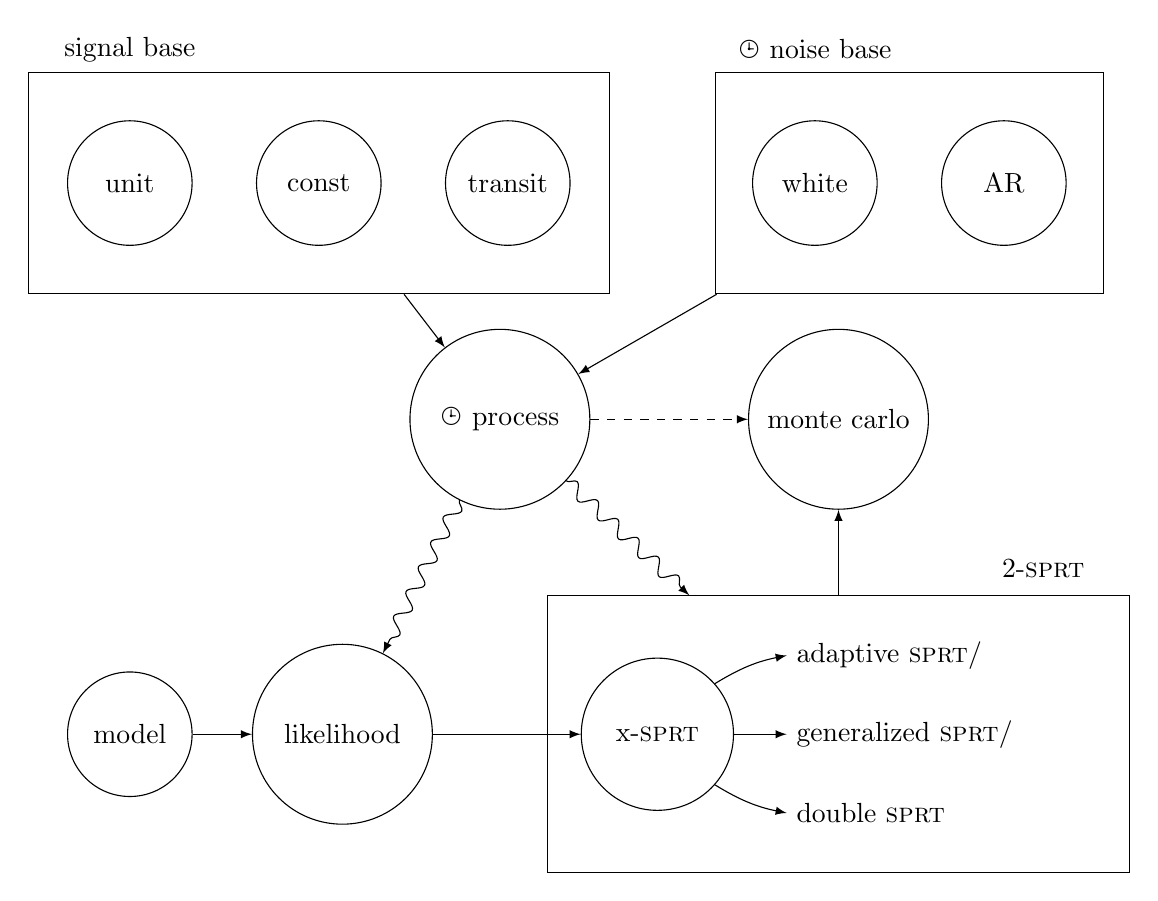
\begin{tikzpicture}[
            arrow/.style={->, >=latex},
            %orrow/.style={->, >=latex, dashed},
            orrow/.style={->, >=latex, decorate, decoration={snake, post length=4pt}},
            sprt/.style={align=left, text width=110pt},
            box/.style={inner sep=0pt, minimum width=210pt, minimum height=80pt},
            space/.style={inner sep=0pt, minimum size=55pt, text width=50pt, align=center},
            subspace/.style={inner sep=0pt, minimum size=45pt, text width=40pt, align=center},
            supspace/.style={inner sep=0pt, minimum size=65pt, text width=60pt, align=center}
        ]
        % ~~ Signals ~~
        \node[draw, rectangle, box] (sbase)   at (-4.3, 6.0) { }; \node at (-6.7, 6.0 + 1.7) {signal base};
        \node[draw, circle, subspace] (sunit)    at (-6.7, 6.0) {unit};
        \node[draw, circle, subspace] (sconst)   at (-4.3, 6.0) {const};
        \node[draw, circle, subspace] (stransit) at (-1.9, 6.0) {transit};
        % ~~ Noises ~~
        \node[draw, rectangle, box, minimum width=140pt] (nbase) at (+3.2, 6.0) { }; \node at (+2.0, 6.0 + 1.7) {\clock{} noise base};
        \node[draw, circle, subspace] (nwhite)   at (+2.0, 6.0) {white};
        \node[draw, circle, subspace] (nautoreg) at (+4.4, 6.0) {AR};
        % ~~ Process ~~
        \node[draw, circle, supspace] (process)  at (-2.0, 3.0) {\clock{} process};
        % ~~ Model and Observers ~~;
        \node[draw, circle, subspace] (model) at (-6.7, -1.0) {model};
        \node[draw, circle, supspace, minimum size=65pt] (likelihood) at (-4.0, -1.0) {likelihood};
        \node[draw, rectangle, box, minimum height=100pt] (observer) at (2.3, -1.0) { }; \node at (4.9, -1.0 + 2.1) {2-\textsc{sprt}};
        \node[draw, circle, space] (twosprt) at (-0.0, -1.0)  {x-\textsc{sprt}};
        \node[sprt] (asprt) at (3.7, -0.0) {adaptive \textsc{sprt}/$\medstar $};
        \node[sprt] (gsprt) at (3.7, -1.0) {generalized \textsc{sprt}/$\medstar $};
        \node[sprt] (dsprt) at (3.7, -2.0) {double \textsc{sprt}};
        % ~~ Monte-Carlo ~~
        \node[draw, circle, supspace] (montecarlo) at (2.3, 3.0) {monte carlo};
        % ~~ Arrows ~~
        \draw[arrow] (sbase)    edge (process);
        \draw[arrow] (nbase)    edge (process);
        \draw[arrow] (model)    edge (likelihood);
        % ~~ Observer arrows ~~
        \draw[orrow] (process) -- (likelihood);
        \draw[orrow] (process) -- (observer);
        % ~~ More Arrows ~~
        \draw[arrow] (likelihood)    edge (twosprt);
        \draw[arrow, dashed] (process) edge (montecarlo);
        \draw[arrow] (observer) edge (montecarlo);
        \draw[arrow] (twosprt)  edge[bend left=10]  (asprt.west);
        \draw[arrow] (twosprt)  edge                (gsprt.west);
        \draw[arrow] (twosprt)  edge[bend right=10] (dsprt.west);
    \end{tikzpicture}
    \end{center}

\subsection*{Fundamental structures.}

\begin{itemize}
	\item Signals: \texttt{unit\_signal}, \texttt{constant\_signal}, \texttt{transitionary\_signal}.
	\item Noises: \texttt{white\_noise}, \texttt{auto\_regressive\_noise}.
	\item Processes: \texttt{process}.
	\item Hypotheses models: \texttt{model}.
	\item Decision rules: \texttt{adaptive\_sprt}(\texttt{\_star}), \texttt{generalized\_sprt}(\texttt{\_star}), \texttt{double\_sprt}.
\end{itemize}

\subsection*{CRTP structures.}

The following are the base abstract CRTP structures:
\begin{itemize}
    \item \texttt{timed}: for timed random sequences, denoted with \clock{} on the diagram.
    \item \texttt{signal\_base}: for signals.
    \item \texttt{noise\_base}: for noises.
    \item \texttt{observer}: for observers of \texttt{process}, denoted with $\rightsquigarrow $ on the diagram.
    \item \texttt{two\_sprt}: for SPRT-based decision rules.
\end{itemize}

%\subsection*{Auxiliary structures.}


\section*{Project \texttt{simulator}.}

Now to the actual program. The description of simulations to be run are stored in \texttt{config}.
More specifically, it contains information necessary to create
\begin{itemize}
    \item \texttt{signal};
    \item \texttt{noise};
    \item \texttt{monte\_carlo};
    \item list of \texttt{two\_sprt}'s;
    \item list of \texttt{run}'s to be performed. 
\end{itemize}
%
The description of simulation, \texttt{run}, contains information about
\begin{itemize}
    \item \texttt{model};
    \item list of \texttt{simulation\_pair}'s;
    \item list of thresholds for each \texttt{two\_sprt}.
\end{itemize}

A \texttt{simulation\_pair} is the pair of signal strengths: the one simulated in the \texttt{process}, denoted here with $\nu $; and the one analyzed by the \texttt{two\_sprt}, which we will denote with $\lambda $.
Regardless of the provided list of \texttt{simulation\_pair}'s, there are four mandatory pairs to assess basic operating characteristics, summarized in this table:
\begin{center}
    \renewcommand{\arraystretch}{1.4}
    \begin{tabular}{ r | c | c | }
        \multicolumn{1}{r}{}
            & \multicolumn{1}{c}{$\lambda = \mu _0$}
            & \multicolumn{1}{c}{$\lambda = \mu _1$}           \\ \cline{2-3}
        $\nu = \mu _0$  & $\ESS _{\mu _0}$  & $\PMS $          \\ \cline{2-3}
        $\nu = \mu _1$  & $\PFA $           & $\ESS _{\mu _1}$ \\ \cline{2-3}
    \end{tabular}
\end{center}


\end{document}
